\section{Projection to QFT and Morphic Fusion/Fission Dynamics}
\label{sec:morphic_projection}

\paragraph{Projection.} Let $\psi_k\in\mathcal C_\Psi$ be a morphic coherence knot
stabilized under the Grace operator $\mathcal G$. Given a measurement-resonant
lattice $\mathcal L$ and a projection functor $\pi: \mathcal C_\Psi\to\mathcal C_{\mathrm{QFT}}$,
the projection is defined by the grace-resonant rule
\[\pi(\psi_k) = \begin{cases}
P(\psi_k) & \text{if } \langle \psi_k, \mathcal L \rangle_{\mathcal G} > \tau,\\
\varnothing & \text{otherwise,}\end{cases}\]
where $\langle\cdot,\cdot\rangle_{\mathcal G}$ is the $\mathcal G$-resonant inner
product and $\tau$ a theory-native threshold. Implementation is provided in
`structures/morphic_algebra.py` (theory-only).

\paragraph{Fusion.} For $\psi_a,\psi_b\in\mathcal C_\Psi$, fusion is a monoidal
operation $\psi_f=\mathcal F_{\mathcal G}(\psi_a,\psi_b)$ permitted when: (i) phase-lock
within a $\phi$-harmonic tolerance, (ii) recursion levels overlap, and (iii) the
admittance condition $\mathcal G(\psi_f)\ge\min(\mathcal G(\psi_a),\mathcal G(\psi_b)) - \epsilon$
holds. A minimal theory implementation is included.

\paragraph{Fission.} For $\psi_k$, fission $(\psi_1,\psi_2)=\mathcal S_{\mathcal G}(\psi_k)$
occurs when a stress functional exceeds a threshold, producing two children with
partitioned coherence and slightly increased decoherence. Theory-only routines
are provided for demonstrations and figures.

\paragraph{Survival under Stochastic Devourer Pressure.} Modeling recursion-time
evolution via $\mathrm d\psi_k(t) = \lambda_k\,\mathrm dt + \sigma_k\,\mathrm dW_t$ with
$\lambda_k = \mathcal G(\psi_k) - \mathcal D(\psi_k)$ yields a survival distribution
\[P_s(k,t)=\Phi\!\left(\frac{\psi_k(0)+\lambda_k t}{\sigma_k\sqrt t}\right)
\exp\!\left(-\frac{2\lambda_k\,\psi_k(0)}{\sigma_k^2}\right),\]
where $\Phi$ is the Gaussian CDF.

\paragraph{Visualization.} A theory-only simulation of survival under stochastic
devourer pressure (absorbing boundary at zero) is provided; see the survival
curve below.
\\
\noindent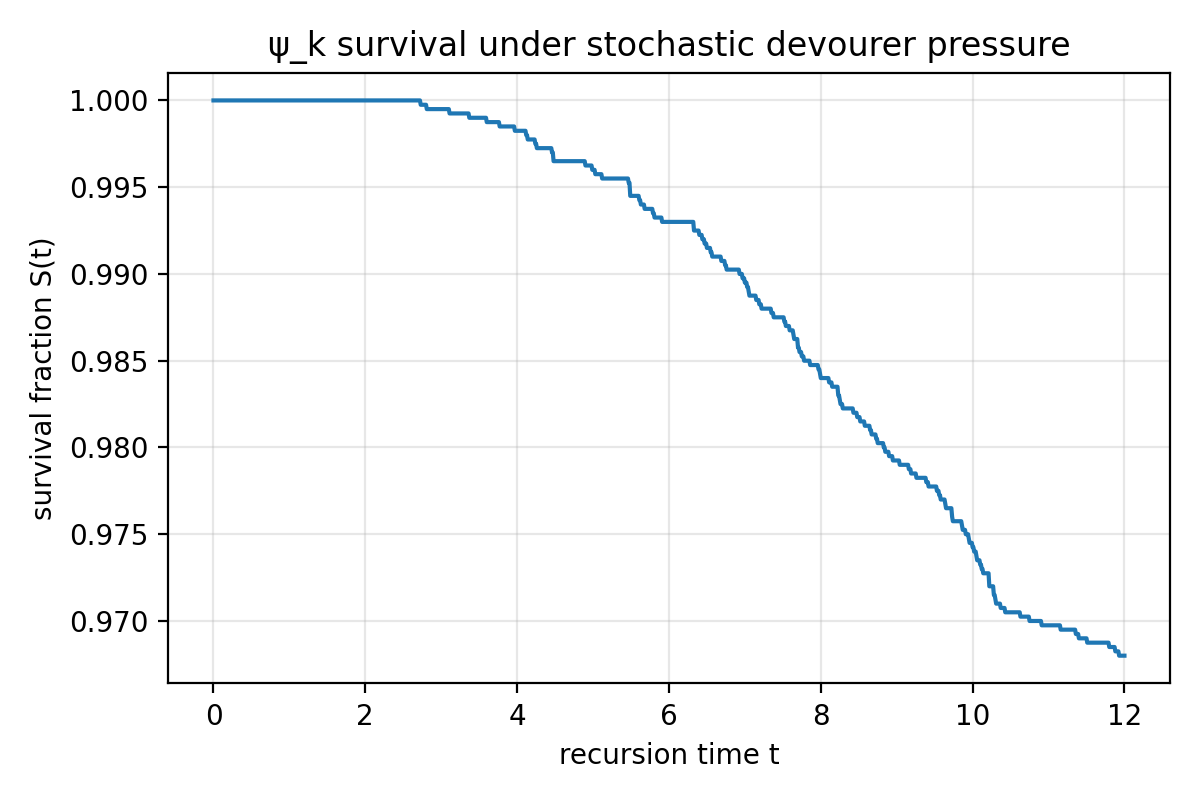
\includegraphics[width=0.75\linewidth]{figures/morphic_survival_curve.png}

\paragraph{FSCTF$\to$QFT Bridge (Sketch).} Mapping $\psi_k$ to localized field
excitations defines a Lagrangian density with self-recursive potential;
fusion corresponds to interaction vertices with couplings given by morphic
inner products; collapse corresponds to decay channels with entropy leakage.
The Grace field plays the role of a coherence-stabilizing vacuum scalar.

\paragraph{Recursive Potential Wells.} Slices of the recursive potential $V(\phi,\mathcal G)$
for different recursion depths $d$ illustrate identity wells and barriers:
\\
\noindent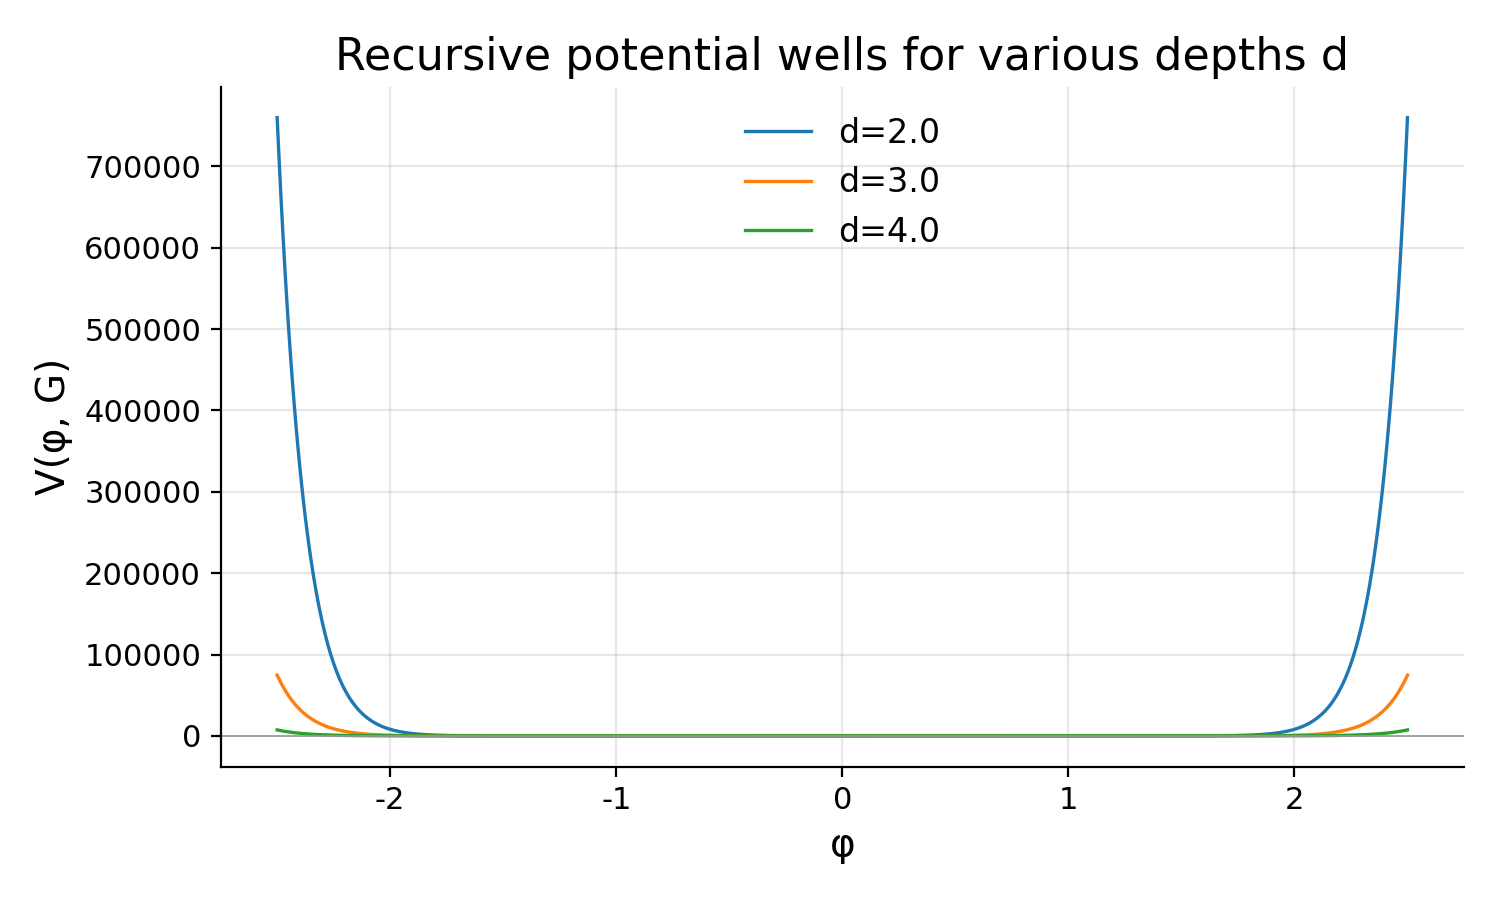
\includegraphics[width=0.85\linewidth]{figures/recursive_potential_wells.png}


